\section{Experiments} \label{sec:experiments}

We now describe the results of three simple experiments designed to
evaluate the suitability of particular planners (FF, SGPLAN, and an ad-hoc
implementation of GraphPlan) in our two NLG domains. As a first impression,
our results indicate that planning is a promising tool for both domains. In
the GIVE domain, SGPLAN 5.2.2 computes a domain plan from the initial state
to the goal in 0.3 seconds, which is fast enough for moderately-sized
problems instances in the application.\footnote{All runtimes were
  measured on a Pentium 4 CPU running at 3 GHz. Java programs were allowed
  to ``warm up'', i.e.\ the planner was run five times and the first four
  measurements discarded to ensure that the JVM had just-in-time compiled
  all relevant bytecode.}
In the sentence generation domain, FF dramatically outperforms the best
previously known algorithm for the same problem (a reimplementation of
\cite{Stone2003a}), although the latter is a greedy search algorithm with a
heuristic that is hand-tailored to the domain.

We also observe that although FF manages the search for a plan very
efficiently, it spends comparatively large amounts of time computing
instantiations of predicates and actions, most of which are then never used
during the search. As a result, FF's ``grounding time'' dominates its
overall planning time, leading to some conflicting results. Our experiments
below seek to improve our understanding of this situation.


\subsection{Experiment 1: Sentence generation}
\label{sec:exper-1:-sent}

In the first experiment, we generate a series of sentence generation
problems which require the planner to compute a plan representing the
sentence ``Mary likes the Adj$_1$ \ldots Adj$_n$ rabbit.''  Each problem
instance assumes a certain number $m$ of rabbits that were distinguished by
$n \leq m$ different properties, such that all $n$ properties are required
to distinguish the target referent from all other rabbits.  The $n$
properties are realized as $n$ different adjectives, in any order.  This
setup allows us to control the plan length (a plan with $n$ properties will
have length $n+4$) and the universe size (the universe will contain $m+1$
individuals in addition to the differently-typed individuals used to encode
the grammar).

\begin{figure}
  \centering
  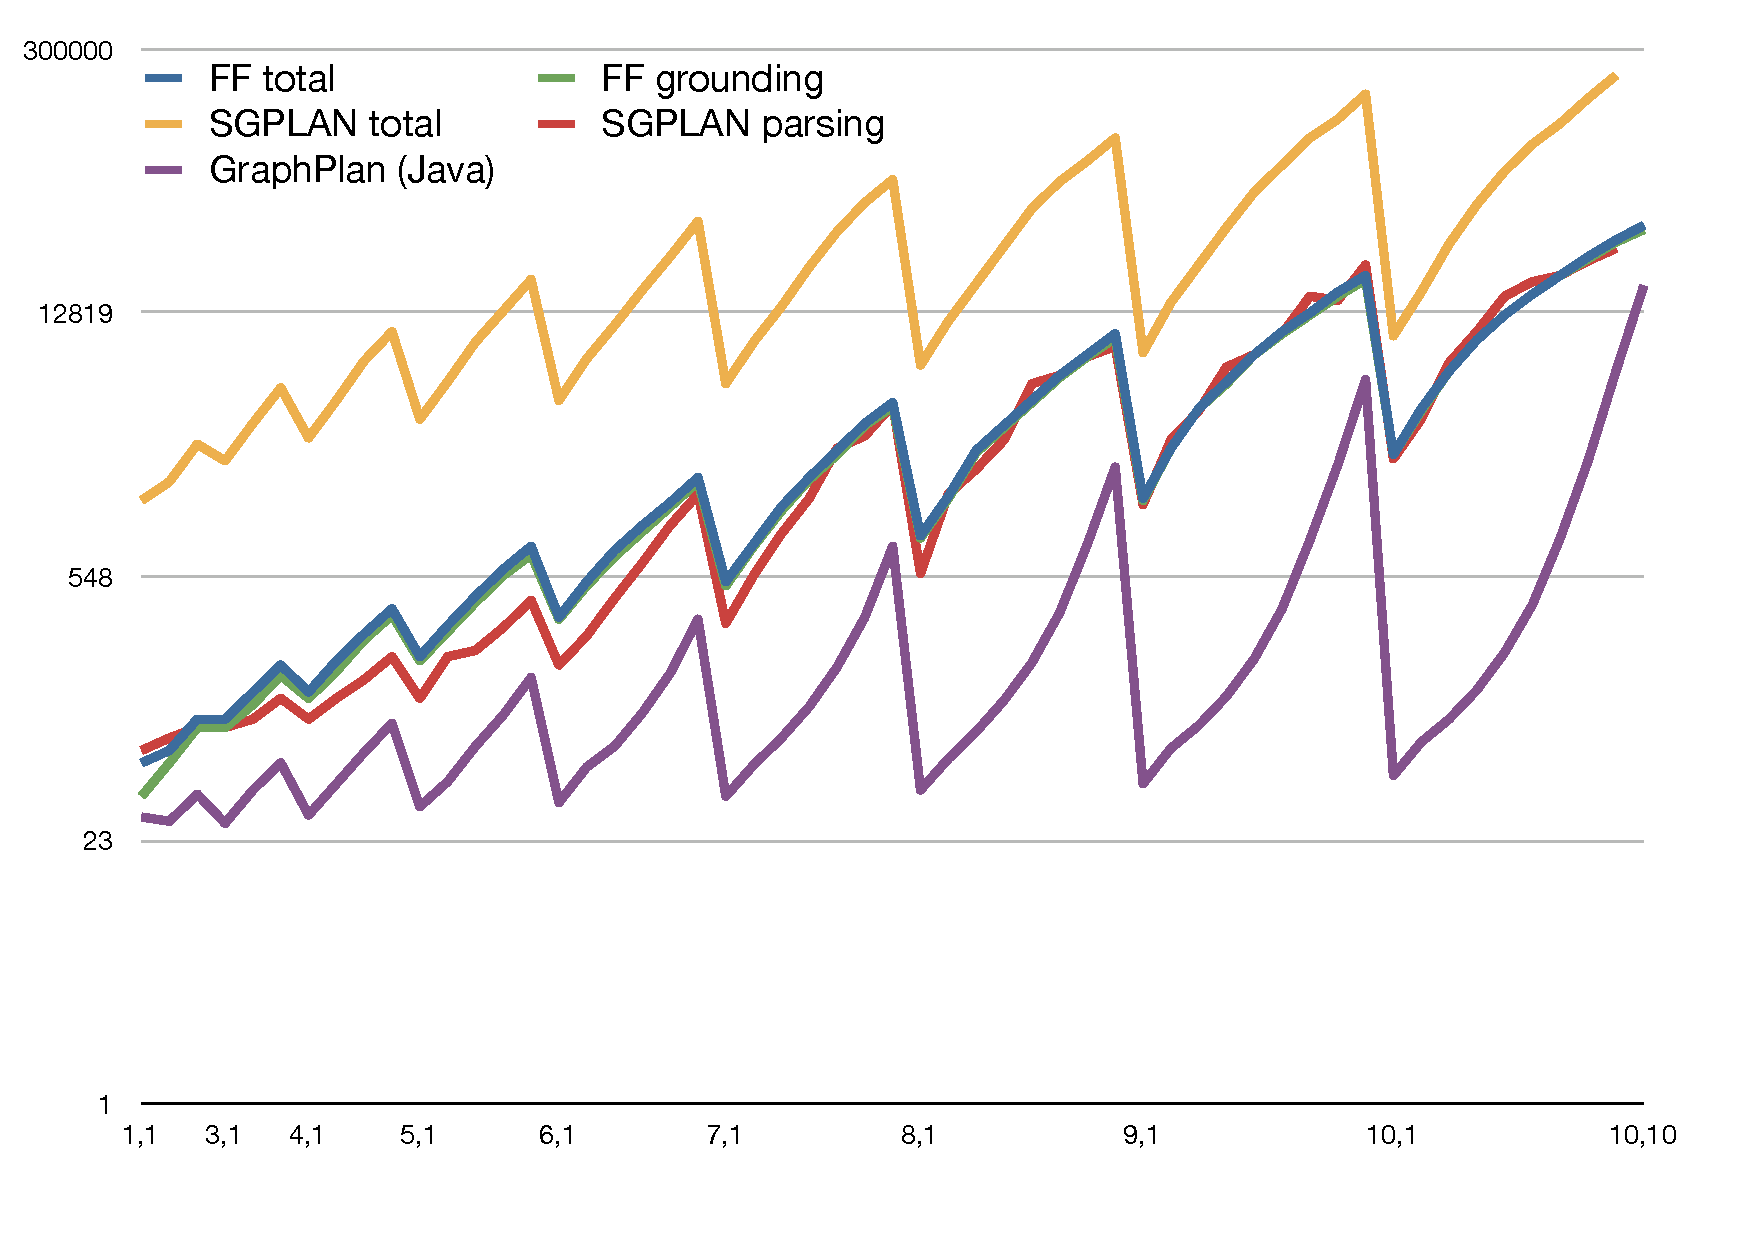
\includegraphics[width=1\columnwidth]{pic-runtime-modifiers-with-sgplan}
  \caption{Runtimes (in ms) in the sentence generation domain.  The
    horizontal axis represents parameters $(m,n)$ from $(1,1)$ to
    $(10,10)$ in lexicographical order.}
  \label{fig:runtimes-crisp}
\end{figure}

The results of this experiment are shown in
Figure~\ref{fig:runtimes-crisp}. The input parameters $(m,n)$ are plotted
(in lexicographic order) on the horizontal axis and the runtime is shown in
milliseconds on the vertical axis. These results reveal a number of
interesting insights. First, FF significantly outperforms
SGPLAN in this domain.\footnote{Experiments with SGPLAN use a
 pre-release version of SGPLAN, kindly provided by Chih-Wei Hsu. The
 release version of SGPLAN 5.2.2 had a bug, causing it to crash on some
 instances.}
Second, FF's runtime is dominated by its initial grounding step, in which
it computes the ground instances of all predicates and actions used in the
planning problem to avoid unnecessary instantiations during search. In
particular, the ratio of grounding time to total runtime is generally above
85\%, and rises to above 99\% at $m=11$, which is still a small universe in
this application.\footnote{The
  ``grounding'' time reported here is what FF reports as ``time spent:
  instantiating action templates''.} 

In fact, FF spends so much time on grounding that it is consistently
outperformed by an ad-hoc Java implementation of GraphPlan which only
computes instances of predicates and actions as they are discovered,
while the planning graph is being built -- despite the fact that FF is
consistently much faster as far as pure search time is concerned.
Looking at the difference from a different angle, FF's performance is
much more sensitive to the domain size: if we fix $n=1$, FF takes 60
ms to compute a plan at $m=1$, but 2.4 seconds (for the same plan) at
$m=10$; our GraphPlan implementation takes 30 ms at $m=1$ and still
only 50 ms at $m=10$.  Conversely, GraphPlan's runtime grows much
faster with the plan size (i.e., with growing values of $n$ for a
fixed $m$).  Larger (but still realistically-sized) instances of the
sentence generation problem are still problematic for the planners we
tested.



\subsection{Experiment 2: Minimal GIVE worlds}
\label{sec:exper-2:-minim}

In the second experiment, we evaluate the performance of the planners
on problems arising in the GIVE domain. We construct a series of test
worlds, similar to the one illustrated in
Figure~\ref{fig:give-minimal}. These worlds consist of a $2n$ by $h$
grid of positions, such that there are buttons at positions $(2i-1,1)$
and $(2i,h)$ for $1 \leq i \leq n$. The player starts in position
$(1,1)$ and must press all buttons in order to successfully complete
the game. The world is generated as a GIVE world description, and then
automatically converted into a planning problem as in
Fig.~\ref{fig:give-planning} by the GIVE software.

\begin{figure}
  \centering
  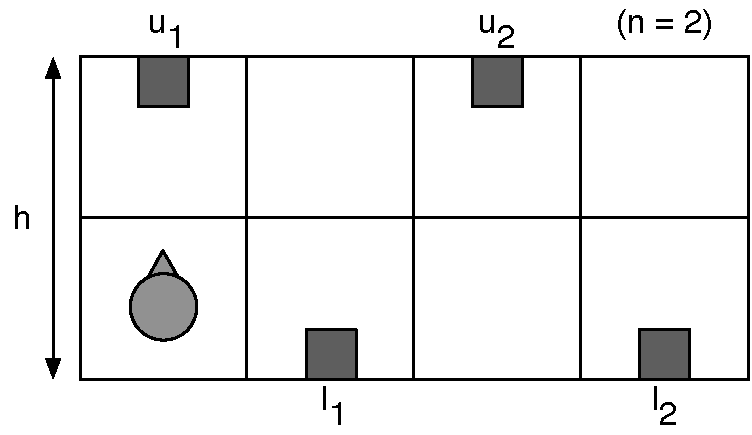
\includegraphics[width=0.8\columnwidth]{pic-buttons}
  \caption{Minimal GIVE world.}
  \label{fig:give-minimal}
\end{figure}

Results for the $h=20$ case, with $n$ ranging from $1$ to $40$, are shown
in Figure~\ref{fig:give-runtime-minimal}.  The most obvious result is that
FF is unable to solve any problems beyond $n=13$ on our experimentation
machine within the memory limit of 1 GB.  SGPLAN, on the other hand, solves
instances beyond $n=40$ without major problems.  The time spent on
grounding is not a major factor in either planner, probably because the
planners need more time to actually compute the plan---for instance, the
optimal plan for the problem $n=40$ has a length of about 1600 steps.

\begin{figure}
  \centering
  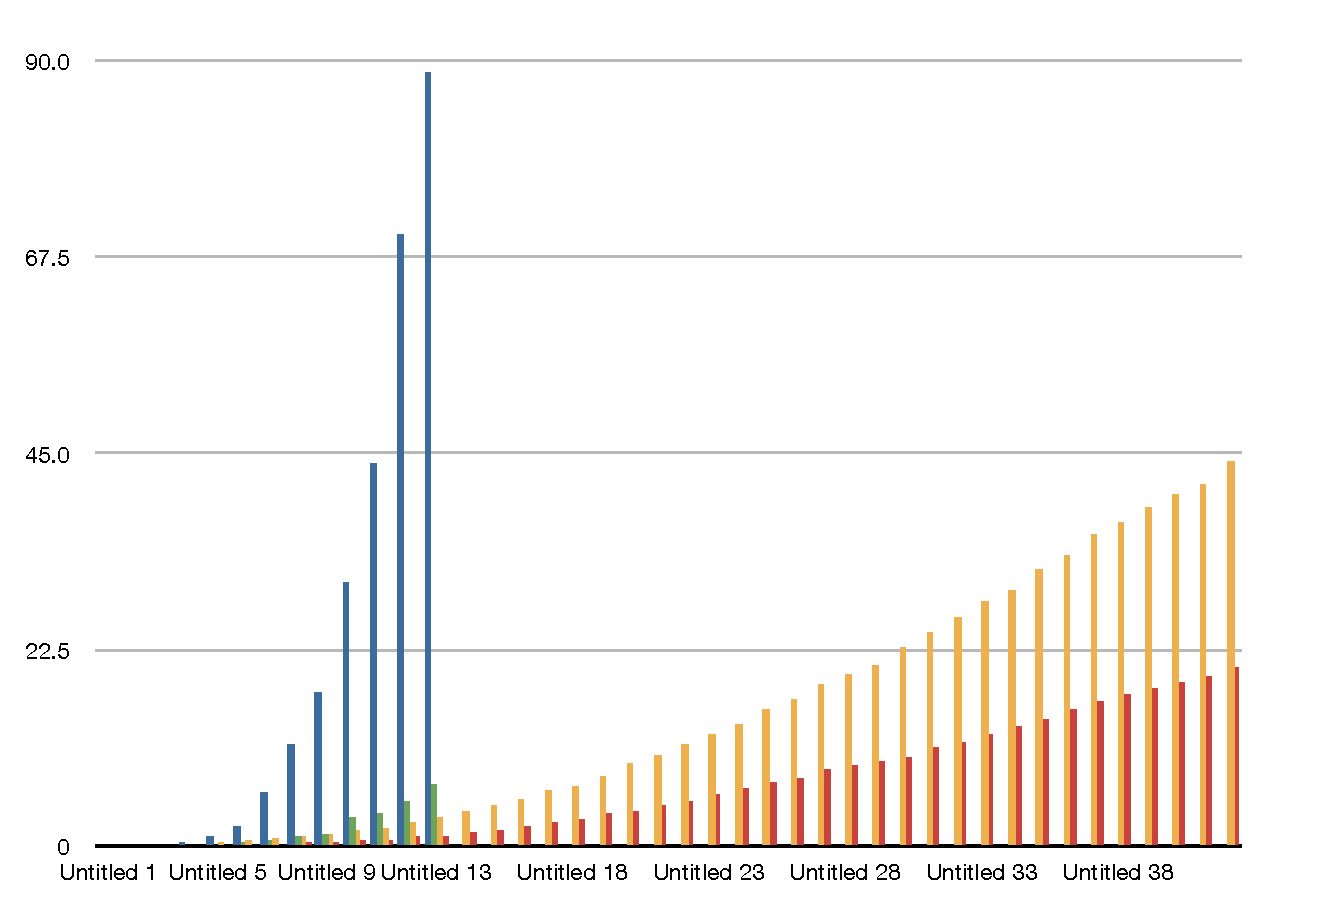
\includegraphics[width=1\columnwidth]{pic-runtime-buttons}
  \caption{Runtimes (in seconds) of FF and SGPLAN on the minimal GIVE
    worlds for $h=20$. The horizontal axis is $n$.}
  \label{fig:give-runtime-minimal}
\end{figure}


\subsection{Experiment 3: GIVE worlds with extra positions}
\label{sec:experiment-3:-give}

In the final experiment, we vary the structure of the GIVE world in order
to judge the effect that universe size has on the planning problem in this
domain.  Starting with the ordinary GIVE world described in Experiment~2,
we add another $w$ by $h$ empty ``junk'' positions to the right of the
minimal world (see Figure~\ref{fig:give-junk}). These new positions are not
actually needed in any plan, but approximate the situation in the actual
GIVE domain, where most grid positions never need to be used. We leave the
initial state and goal untouched. As before, we generate a GIVE world
description and then convert it into a planning problem.

\begin{figure}
  \centering
  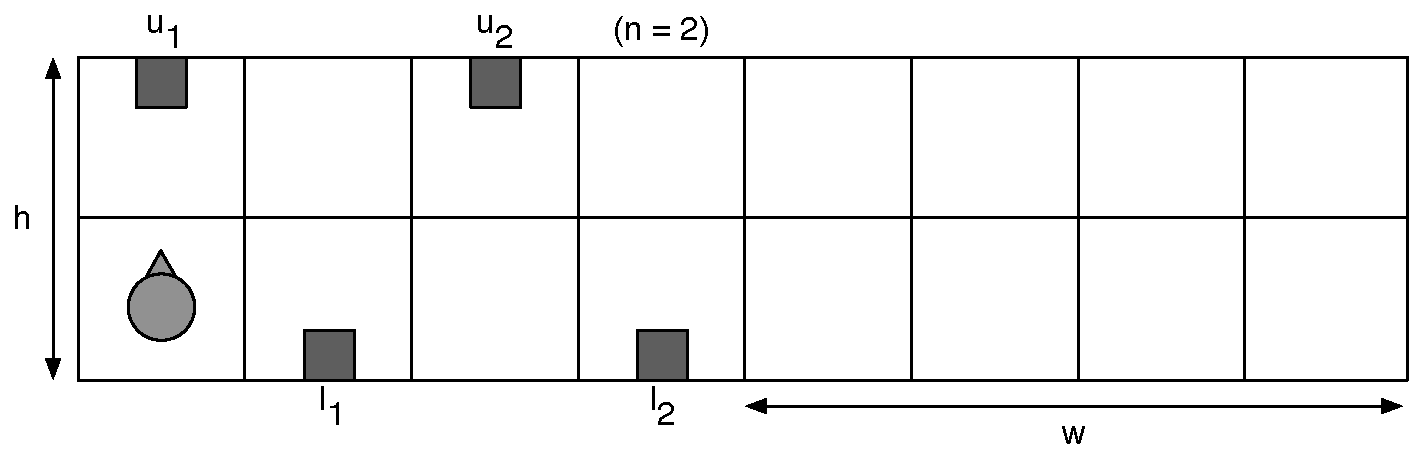
\includegraphics[width=1\columnwidth]{pic-empty-buttons}
  \caption{GIVE world with extra ``junk'' positions.}
  \label{fig:give-junk}
\end{figure}

Results for the $h=20$, $n=5$ case (with $w$ ranging from $1$ to $70$)
are shown in Figure~\ref{fig:give-runtime-junk}. As in Experiment~2,
FF again runs out of memory, this time at $w=17$. SGPLAN happily
solves inputs beyond $w=70$. However, unlike in Experiment 2, both
planners now spend a substantial proportion of their time on
grounding. In SGPLAN, this translates to a ``parsing time'' (which we
assume includes grounding) which grows from 180 ms to 21.7 seconds as
$w$ grows from $1$ to $75$. The rest of the runtime (which also
includes the search time) only grows from 400 ms to 2.3 seconds. This
difference is particularly dramatic given that the actual optimal plan
in each case is an identical plan of about 100 steps. The planning
times for these instances are also concerning since times over a
couple seconds negatively affect the overall response time of the
system, which must react in real time to user actions.

\begin{figure}
  \centering
  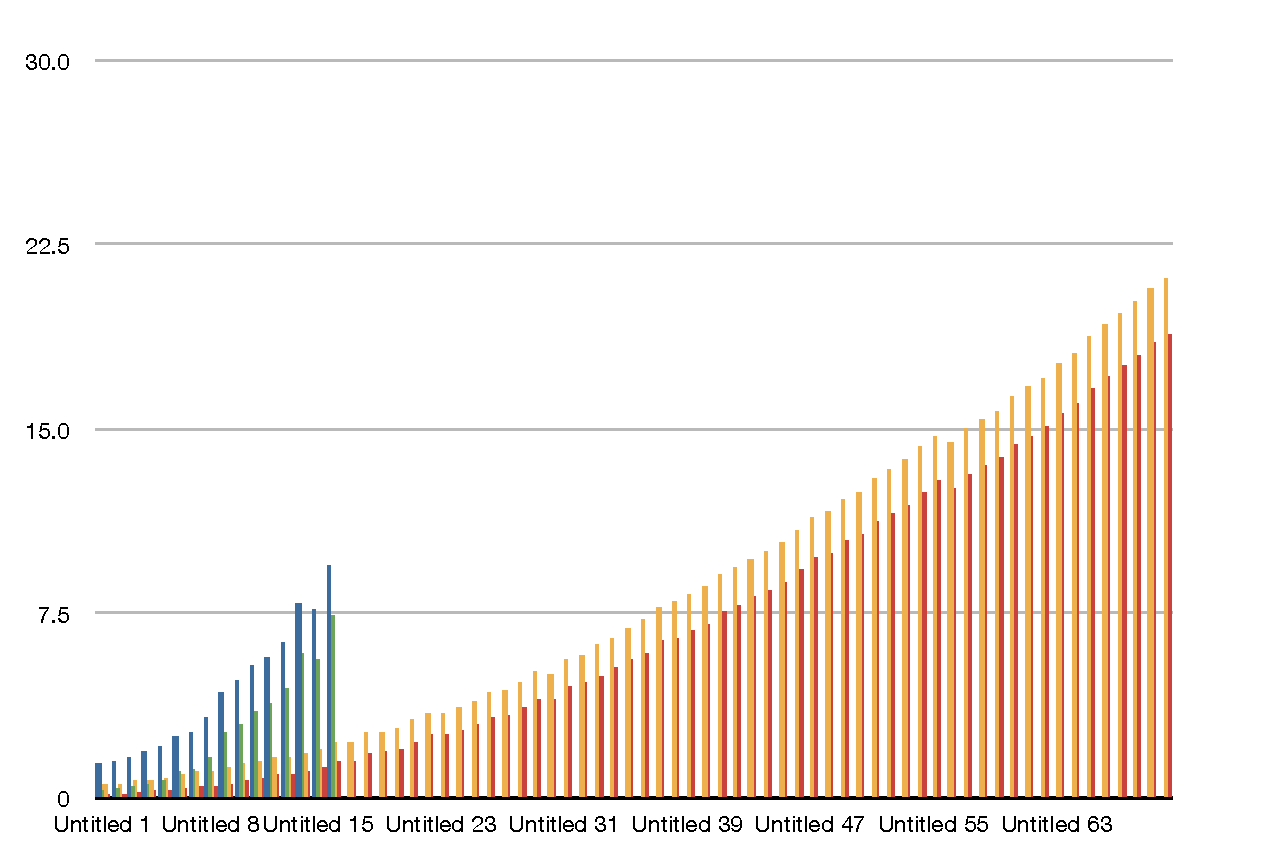
\includegraphics[width=1\columnwidth]{pic-runtime-empty-world}
  \caption{Runtimes (in seconds) of FF and SGPLAN on the GIVE worlds with junk
    positions for $h=20$ and $n=5$. The horizontal axis is $w$.}
  \label{fig:give-runtime-junk}
\end{figure}


%%% Local Variables: 
%%% mode: latex
%%% TeX-master: "experiences"
%%% End: 
